\par Рассмотрим пункт а) (пункт б аналогично)
\par Поле разложения: $\Q(\sqrt[4]{2}, i)$. Степень разложения 8, значит всего 8 автоморфизмов. Каждый автоморфизм задается тем, куда переходят $\sqrt[4]{2}$ и $i$ (каждый из них пеерходит в какой-то другой корень их минимального могочлена. Получаем
\begin{center}
    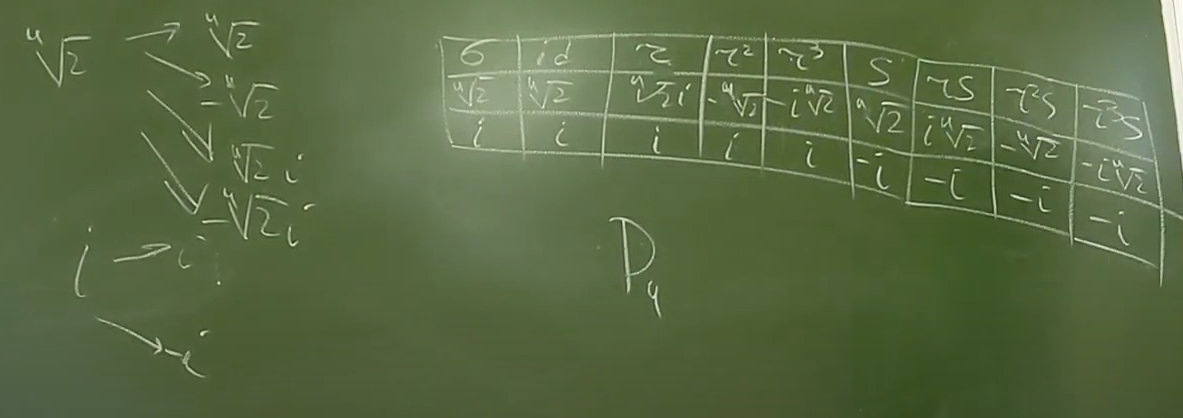
\includegraphics[scale=0.7]{images/automorphisms.png}
\end{center}

\par Что означает табличка: куда переходит $\sqrt[4]{2}$ и $i$. Сначала нашли $r$, посмотрели все комбинации с ним, потом $s$ и посмотрели все комбинации с ним и $r$. Из таблички видим, что структура группы такая же как у $D_4$

\par Для $D_4$ есть нормальная подгруппа порядка 2 из тождественной и центральной симметрии + одна подгруппа порядка 2 $\{id, r^2s\}$. Есть одна подгруппа порядка 4 из поворотов.

\par Остается теперь посмотреть на соответствие полей и подгрупп (TODO чуть поже попробую сделать картинку как на лекции)